\documentclass[varwidth=true, border=2pt]{standalone}

\usepackage{pgfplots}
\pgfplotsset{compat=1.10}
\usepackage{tikz}
\usepgfplotslibrary{fillbetween}
\usepackage{mathtools}

\begin{document}
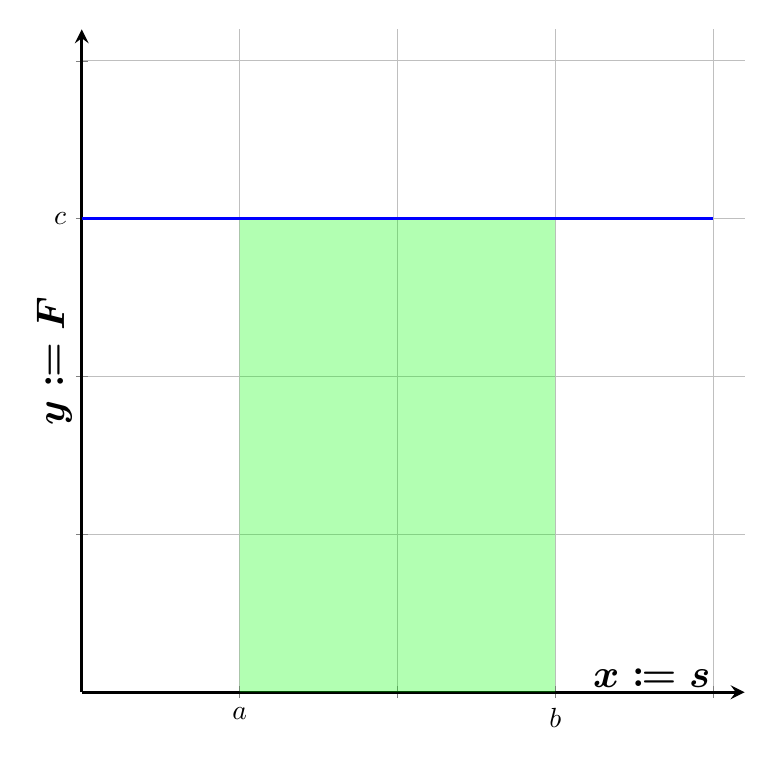
\begin{tikzpicture}
    \begin{axis}[
        width=10cm,
        height=10cm,
        % Grid
        grid = major,
        % size
        xmin= 0,     % start the diagram at this x-coordinate
        xmax= 4.2,   % end   the diagram at this x-coordinate
        ymin= 0,     % start the diagram at this y-coordinate
        ymax= 4.2, % end   the diagram at this y-coordinate
        % Legende
        legend style={
            font=\large\sansmath\sffamily,
            at={(0.5,-0.18)},
            anchor=north,
            legend cell align=left,
            legend columns=-1,
            column sep=0.5cm
        },
        % Ticks
        tick align=inside,
        %minor tick num=3,
        minor tick style={thick},
        scaled y ticks = false,
        xtick={0, 1, 2, 3, 4},
        xticklabels={0, $a$, , $b$,},
        ytick={0, 1, 2, 3, 4},
        yticklabels={, , , $c$, },
        axis lines = middle,
        axis line style = very thick,
        xlabel=$x \coloneqq s$,
        x label style={at={(axis description cs:0.86,0.05)},
                       anchor=north,
                       font=\boldmath\Large},
        ylabel=$y \coloneqq F$,
        y label style={at={(axis description cs:0,0.5)},
                       anchor=south,
                       rotate=90,
                       font=\boldmath\Large},
        ]
      \addplot[domain=0:4, blue, very thick, samples=10, name path=f] {3};
      \path[name path=axis] (axis cs:0,0) -- (axis cs:10,0);
      \addplot[fill=green,
               fill opacity=0.3]
       fill between[of=f and axis,soft clip={domain=1:3}];
    \end{axis} 
\end{tikzpicture}
\end{document}
